\documentclass[10pt,a4paper]{article}
\usepackage[margin=22mm]{geometry}
\usepackage[T1]{fontenc}
\usepackage{lmodern,amsmath,booktabs}
\usepackage{bisse-icons}
\usepackage[colorlinks=true,urlcolor=blue]{hyperref}
\setlength{\parindent}{0pt}
\setlength{\parskip}{7pt}
\begin{document}
{\LARGE\sffamily\bfseries BiSSE event icons}\par
Simple, editable vector graphics for equations, tables and slides.
Blue/open circles denote state 0; vermillion/filled circles denote state 1.
Numerals preserve state identity in grayscale. Time runs from left to right.

\begin{center}
\begin{tabular}{@{}p{57mm}cc@{}}
\toprule
Event & State 0 & State 1\\\midrule
State change & \bisseChange{0}{1} & \bisseChange{1}{0}\\
Speciation: same-state daughters & \bisseSpeciation{0} & \bisseSpeciation{1}\\
Split; upper daughter dies out & \bisseHiddenUpper{0} & \bisseHiddenUpper{1}\\
Split; lower daughter dies out & \bisseHiddenLower{0} & \bisseHiddenLower{1}\\
Extinction & \bisseExtinction{0} & \bisseExtinction{1}\\
Nothing happens & \bisseNothing{0} & \bisseNothing{1}\\\bottomrule
\end{tabular}
\end{center}
\textbf{Meaning of the dashed branch and cross.} A dashed daughter line is
destined to leave no living descendants; the cross denotes extinction.
This summarizes its eventual fate, not necessarily extinction within the
short interval containing the split. A solid daughter is the retained path;
the icon alone does not assert that both solid daughters survive to the present.

\textbf{BiSSE interpretation.} Speciation is $0\to0+0$ or $1\to1+1$;
state change occurs along a lineage, not at the split. The two hidden-split
orientations correspond to the two contributions $\lambda_iD_iE_i$ and
$\lambda_iE_iD_i$ in the backward likelihood equation.

\subsection*{Use directly in Overleaf}
Upload \texttt{bisse-icons.sty} and add \verb|\usepackage{bisse-icons}|.
Commands take a state argument and an optional width:
\begin{verbatim}
\bisseChange{0}{1}
\bisseSpeciation{0}
\bisseHiddenUpper{1}
\bisseHiddenLower[24mm]{0}
\bisseExtinction{1}
\bisseNothing{0}
\end{verbatim}
The default width is 30 mm. All icons share the same bounding box.
For PDF-only use, upload the \texttt{icons} folder and write, for example:
\begin{verbatim}
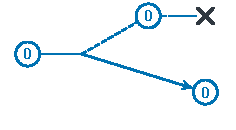
\includegraphics[width=30mm]{icons/hidden-upper-0.pdf}
\end{verbatim}
\textbf{Change the palette:} redefine \texttt{bisseZero} and \texttt{bisseOne}
after loading the package. Open/filled symbols, numbers and extinction crosses
remain informative without relying on hue.
\end{document}
